\section*{Dictionnaire de données}

On identifie les données utiles au système d'information à partir du recueil informel des besoins.

\begin{figure}[!h]
\begin{tabular}{l l l l l l}
%
    \textbf{mnémonique} & \textbf{desc.} & \textbf{type} & \textbf{format} & \textbf{divers} & \textbf{exemple} \\
    adr-livraison            & - & texte    &  - & 50 car.    & 12 rue des blés 92600 Nanterre \\
    adr-facturation          & - & texte    &  - & 50 car.    & 12 rue des blés 92600 Nanterre \\
    id-boulangerie           & - & entier   &  - & séquentiel & 12 \\
    id-client                & - & entier   &  - & séquentiel & 15 \\
    no-commande              & - & entier   &  - & séquentiel & 232 \\
    no-livraison             & - & entier   &  - & séquentiel & 727 \\
    payé                     & - & booléen  &  - & -          & oui \\
    quantité-cmd             & - & entier   &  - & -          & 7 \\
    quantité-livrée          & - & entier   &  - & -          & 5 \\
    type                     & - & texte    &  - & 50 car.    & farine complète \\
%
\end{tabular}
    \caption{\label{DD} Dictionnaire de données}
\end{figure}

\newpage
\section*{Diagramme de Flux}

On identifie les flux d'information en fonction du recueil informel des besoins.

\begin{figure}[!htb]
    \begin{center}
    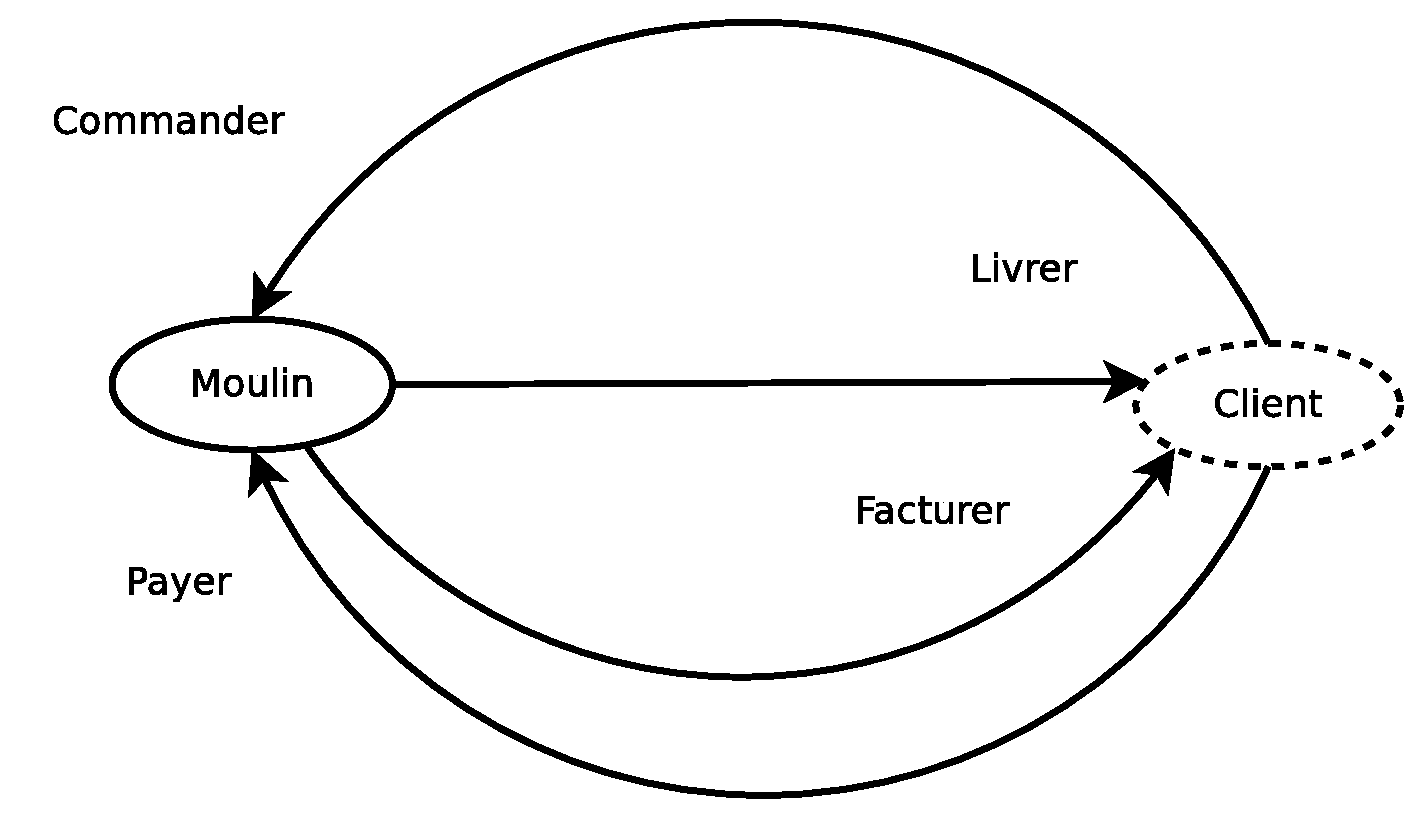
\includegraphics[width=6cm]{images/cc1_df1.eps}
    \caption{\label{cc1_df1} Diagramme de contexte}
    \end{center}
\end{figure}

\begin{figure}[!htb]
    \begin{center}
    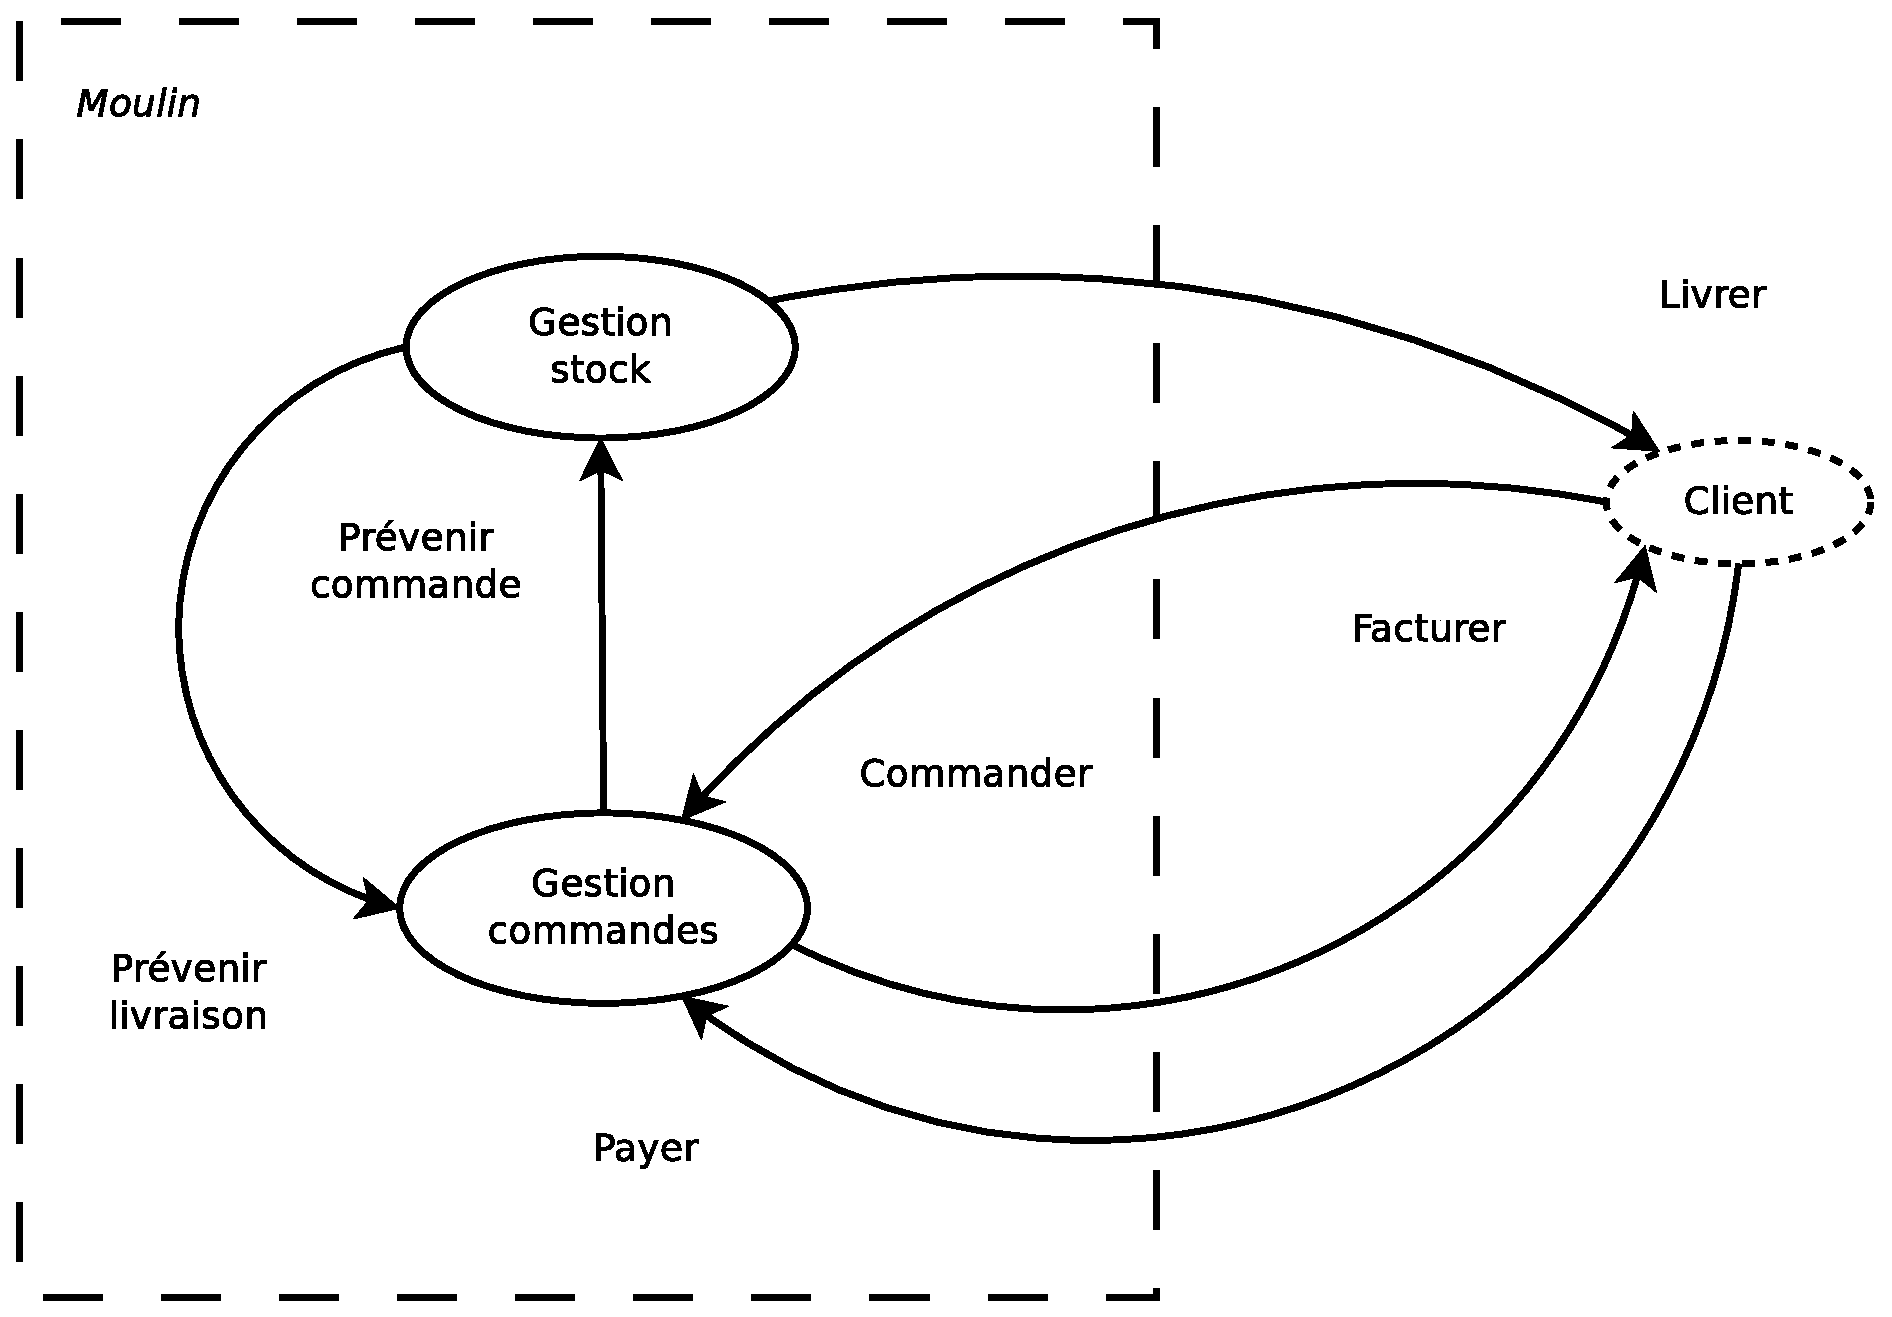
\includegraphics[width=9cm]{images/cc1_df2.eps}
    \caption{\label{cc1_df2} Diagramme d'activité}
    \end{center}
\end{figure}

\begin{figure}[!htb]
    \begin{center}
    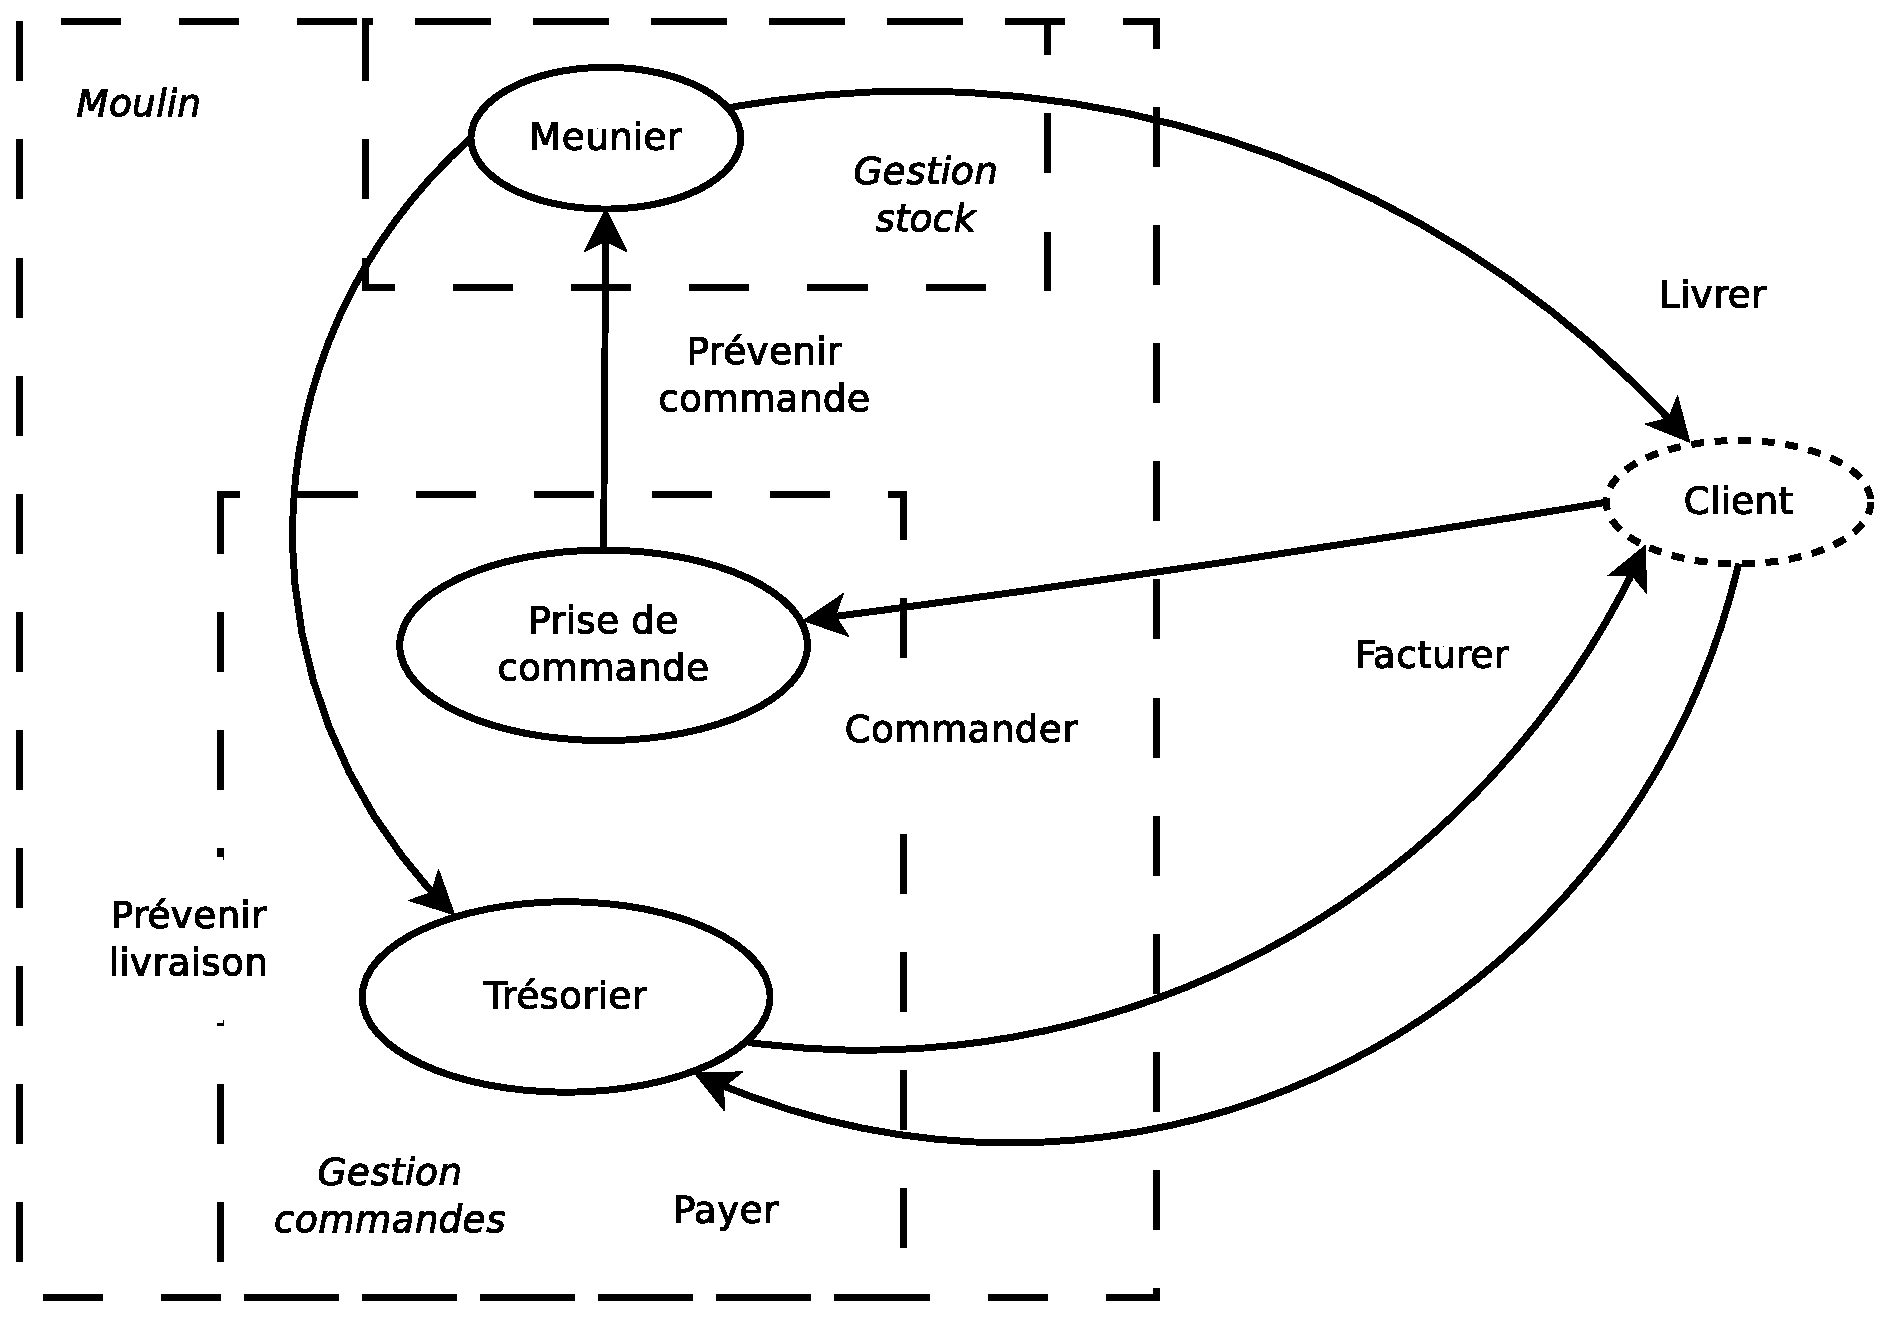
\includegraphics[width=9cm]{images/cc1_df3.eps}
    \caption{\label{cc1_df3} Diagramme de flux}
    \end{center}
\end{figure}

\section*{Matrice des Flux}

À faire à partir du diagramme de flux.

\newpage
\section*{Modèle Concptuel de Communication}

Pour chaque flux d'information du diagramme de flux, on détaille les messages échangés.

\begin{figure}[!htb]
    \begin{center}
    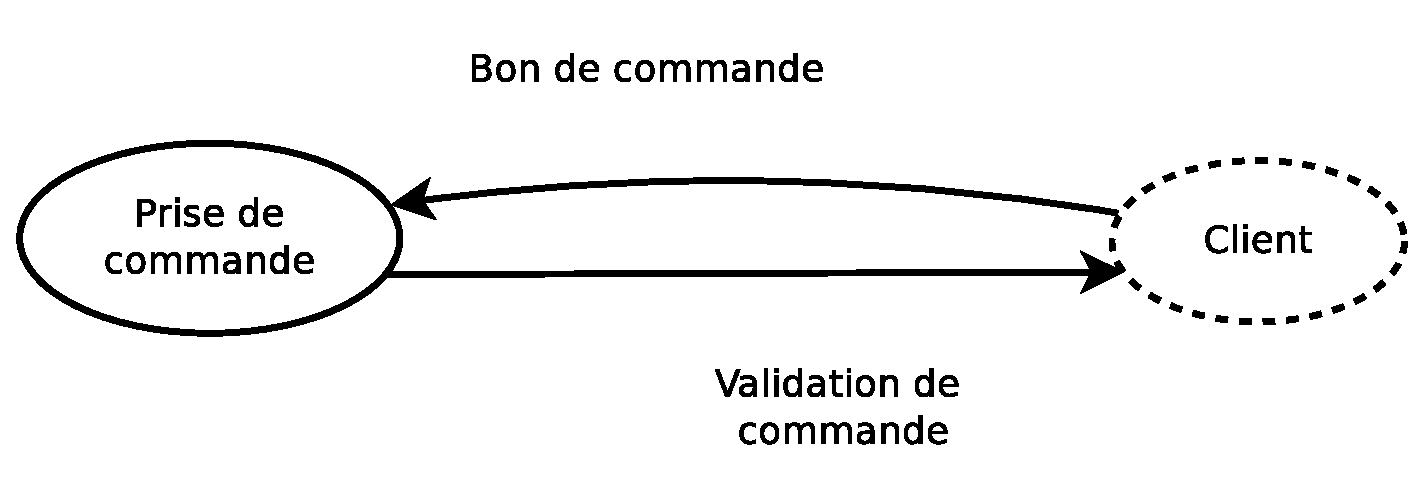
\includegraphics[width=6cm]{images/cc1_mcc1.eps}
    \caption{\label{cc1_mcc1} Commander}
    \end{center}
\end{figure}

\begin{figure}[!htb]
    \begin{center}
    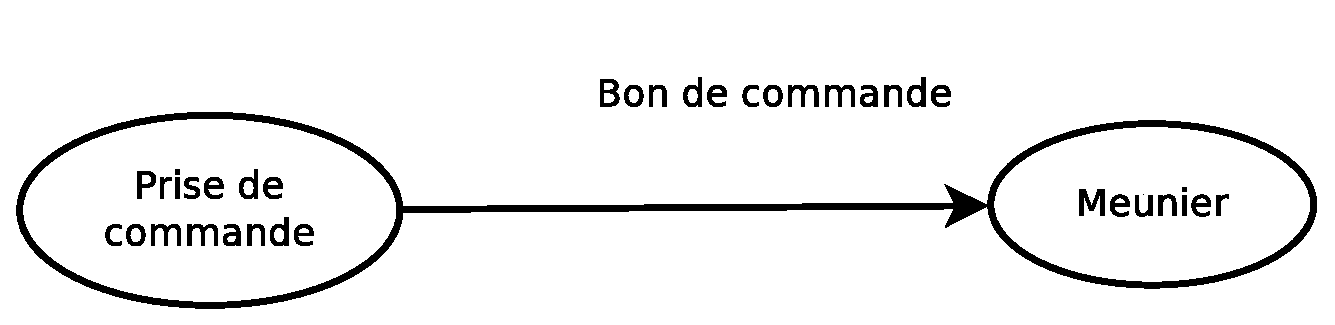
\includegraphics[width=6cm]{images/cc1_mcc2.eps}
    \caption{\label{cc1_mcc2} Prévenir commande}
    \end{center}
\end{figure}

\begin{figure}[!htb]
    \begin{center}
    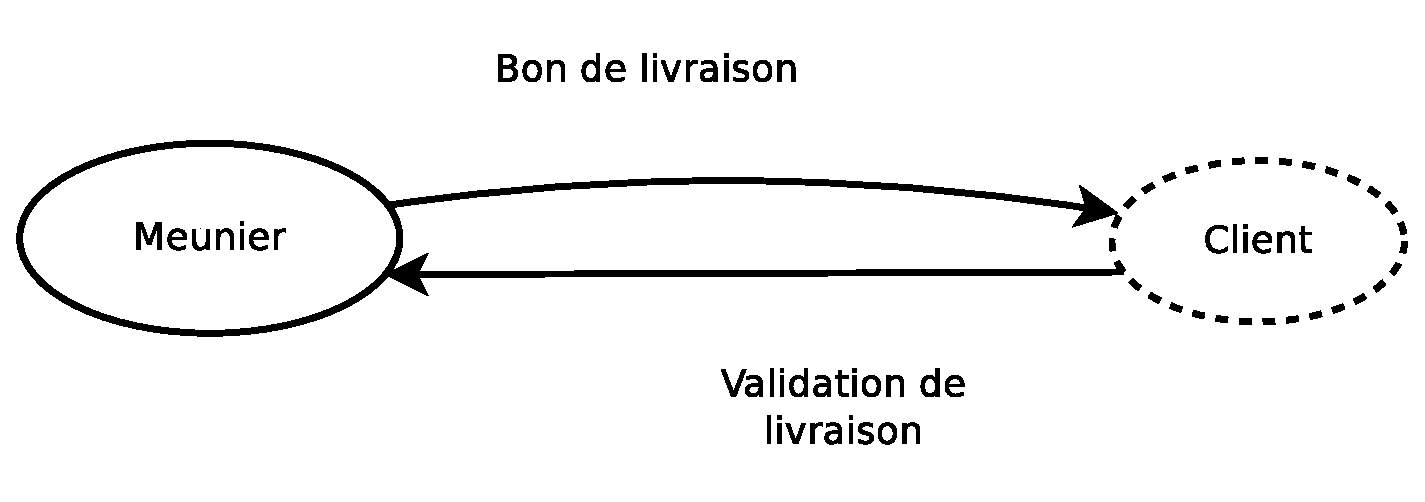
\includegraphics[width=6cm]{images/cc1_mcc3.eps}
    \caption{\label{cc1_mcc3} Livrer}
    \end{center}
\end{figure}

\begin{figure}[!htb]
    \begin{center}
    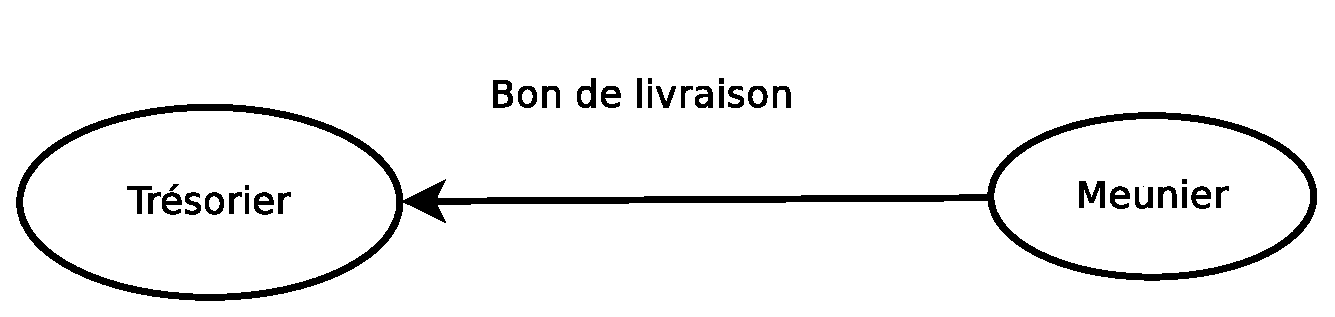
\includegraphics[width=6cm]{images/cc1_mcc4.eps}
    \caption{\label{cc1_mcc4} Prévenir livraison}
    \end{center}
\end{figure}

\begin{figure}[!htb]
    \begin{center}
    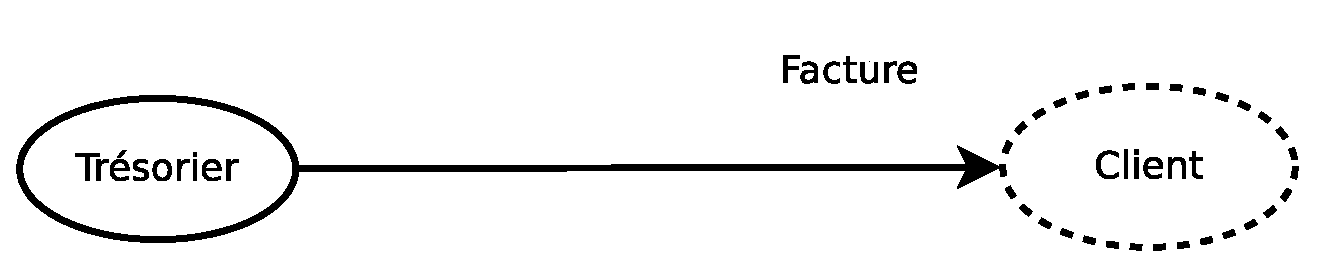
\includegraphics[width=6cm]{images/cc1_mcc5.eps}
    \caption{\label{cc1_mcc4} Facturer}
    \end{center}
\end{figure}

\begin{figure}[!htb]
    \begin{center}
    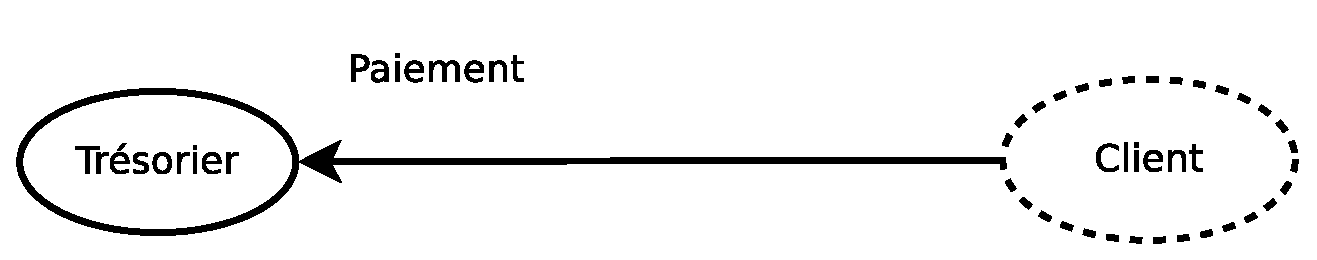
\includegraphics[width=6cm]{images/cc1_mcc6.eps}
    \caption{\label{cc1_mcc4} Payer}
    \end{center}
\end{figure}

\newpage
\section*{Modèle Concptuel de Communication détaillé}

On place affecte maintenant chaque donnée du dictionnaire de données dans le message qui la contient.

\subsubsection*{Bon de commande (Client, Prise de commande)}
\begin{itemize}
    \item no-commande
    \item adr-livraison
    \item adr-facturation
    \item type
    \item qté-cmdée
\end{itemize}

\subsubsection*{Bon de commande validé (Prise de commande, Client)}
\begin{itemize}
    \item no-commande
\end{itemize}

\subsubsection*{Bon de commande (Prise de commande, Meunier)}
\begin{itemize}
    \item no-commande
    \item adr-livraison
    \item adr-facturation
    \item type
    \item qté-cmdée
\end{itemize}

\subsubsection*{Bon de livraison (Meunier, Client)}
\begin{itemize}
    \item no-livraison
    \item no-commande
    \item adr-livraison
    \item type
    \item qté-livré
\end{itemize}

\subsubsection*{Validation de livraison (Client, Meunier)}
\begin{itemize}
    \item no-livraison
\end{itemize}

\subsubsection*{Bon de livraison (Meunier, Trésorier)}
\begin{itemize}
    \item no-livraison
    \item no-commande
    \item adr-livraison
    \item type
    \item qté-livré
\end{itemize}

\subsubsection*{Facture (Trésorier, Client)}
\begin{itemize}
    \item no-livraison
    \item adr-facturation
    \item payé
\end{itemize}

\subsubsection*{Paiement (Client, Trésorier)}
\begin{itemize}
    \item no-livraison
    \item payé
\end{itemize}

\newpage
\section*{Modèle Conceptuel de Données}

En suivant l'ordre des messages du MCC, on place chaque donnée véhiculée par un message dans le MCD. Pour chaque donnée, on se pose la question de l'existance d'une nouvelle entité. Une fois toutes les données placées, on valide notre MCD (formes normales).

\begin{figure}[!htb]
    \begin{center}
    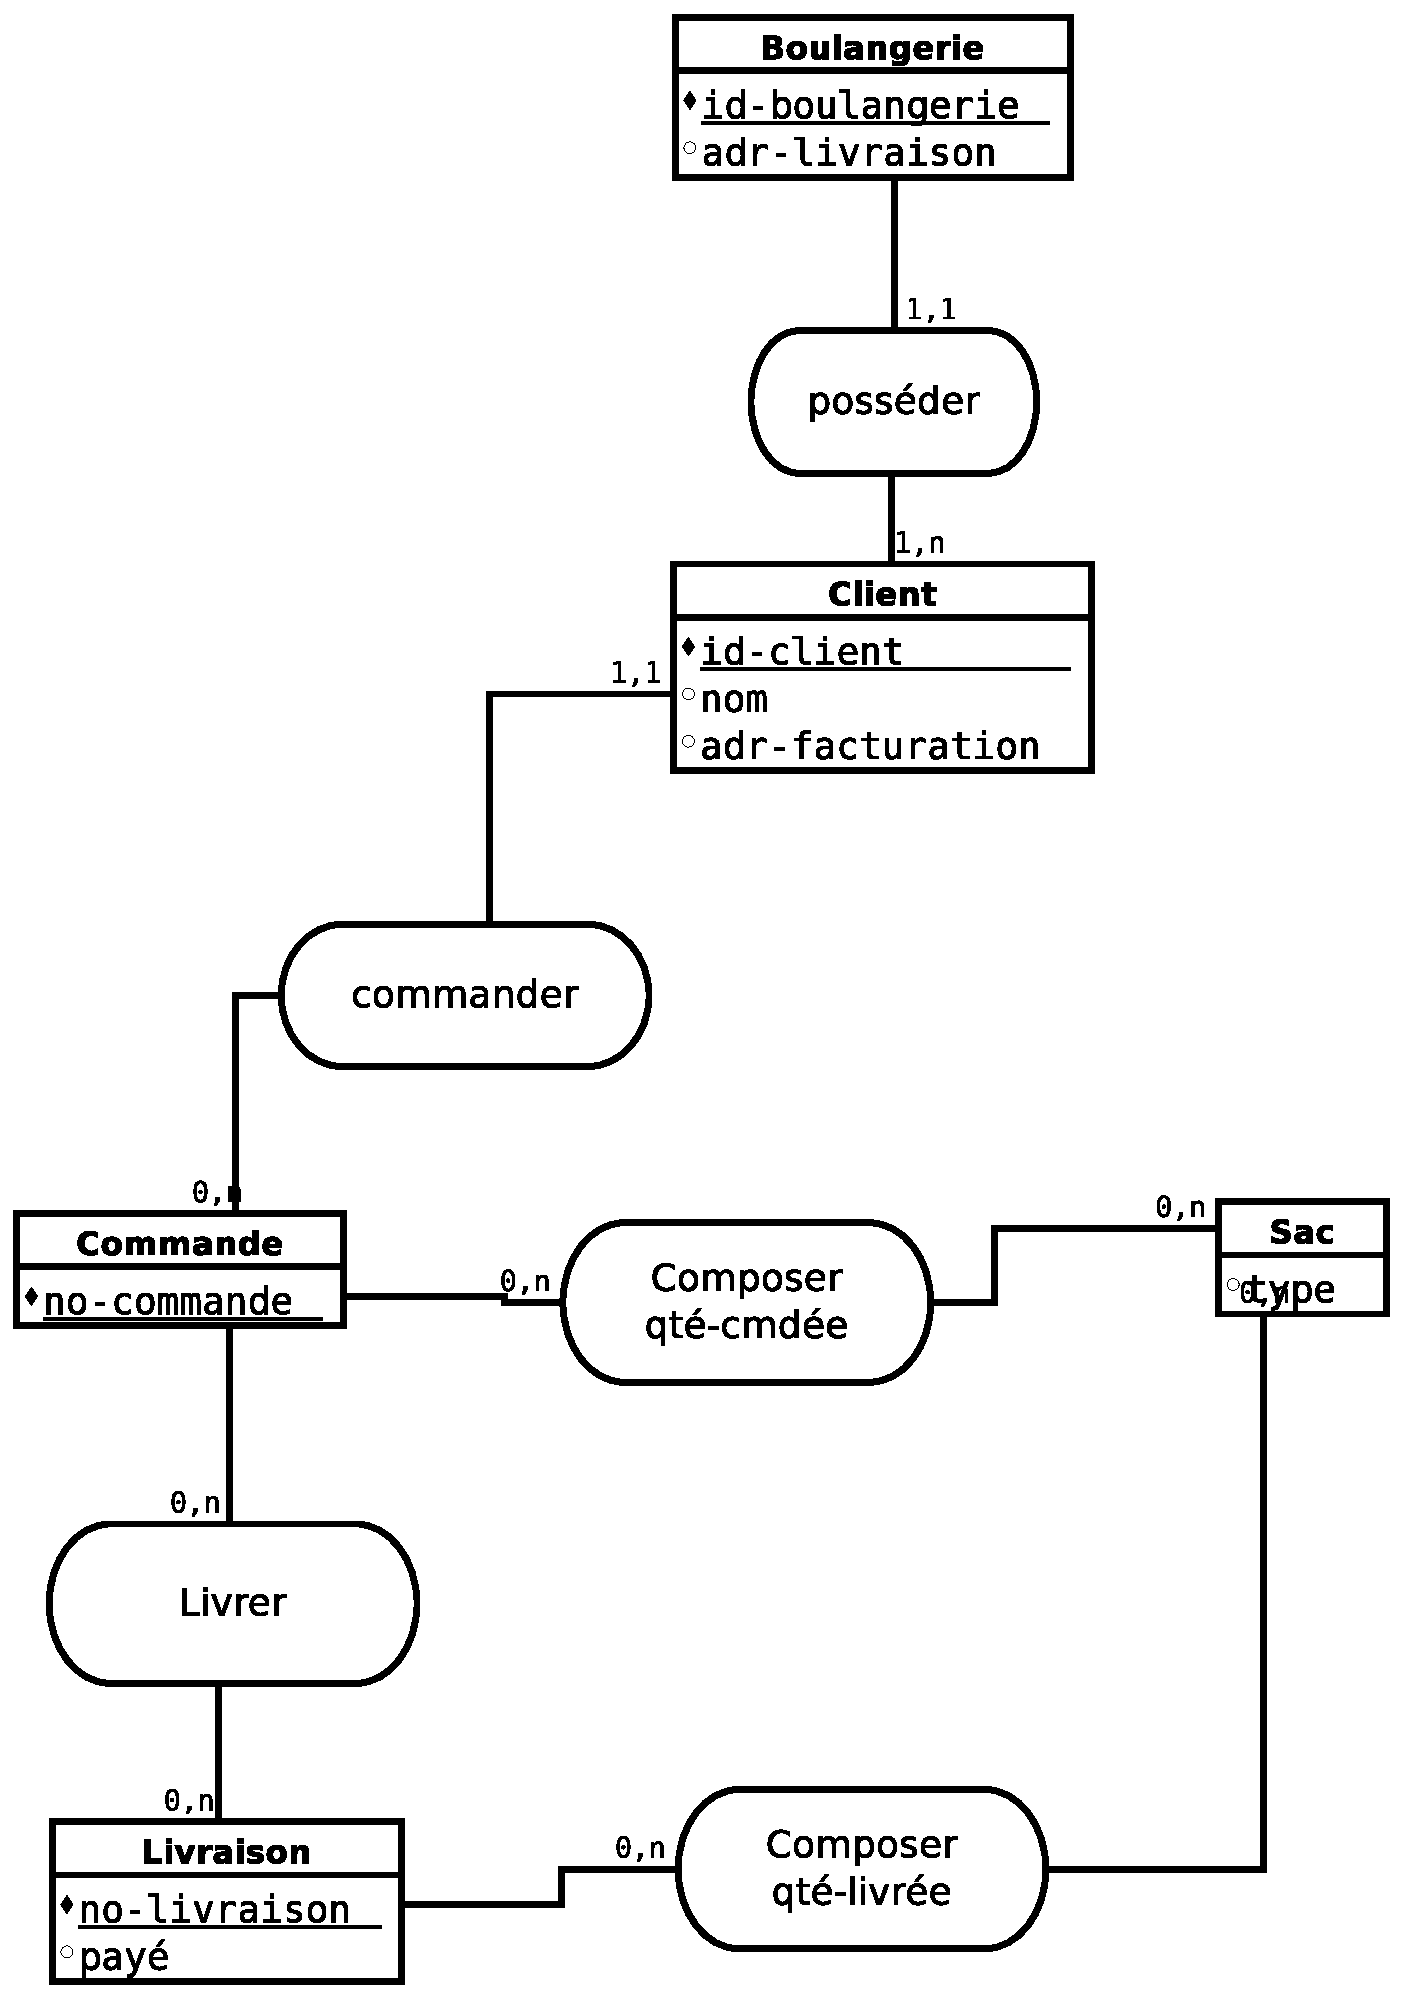
\includegraphics[width=11.5cm]{images/cc1_mcd.eps}
    \caption{\label{cc1_mcd} MCD}
    \end{center}
\end{figure}

\newpage
\section*{Modèle Conceptuel de Traitements}

Pour chaque acteur, on se demande les actions qu'il effectue sur notre système d'information.

\begin{figure}[!htb]
    \begin{center}
    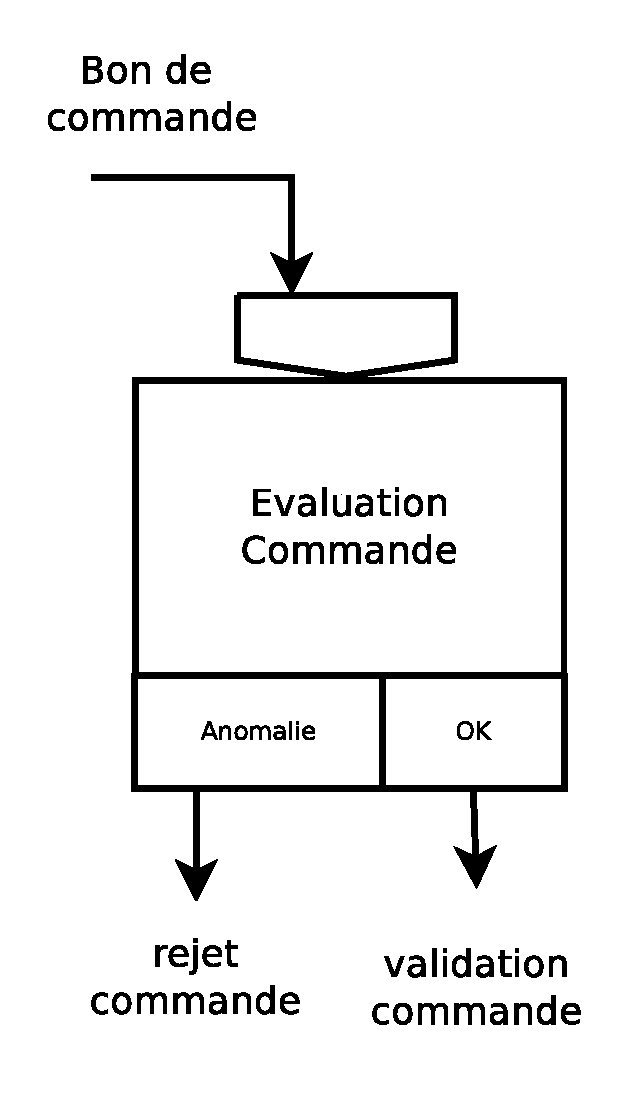
\includegraphics[height=7cm]{images/cc1_mct1.eps}
    \caption{\label{cc1_mct1} Prise de commande  : prendre une commande}
    \end{center}
\end{figure}

\begin{figure}[!htb]
    \begin{center}
    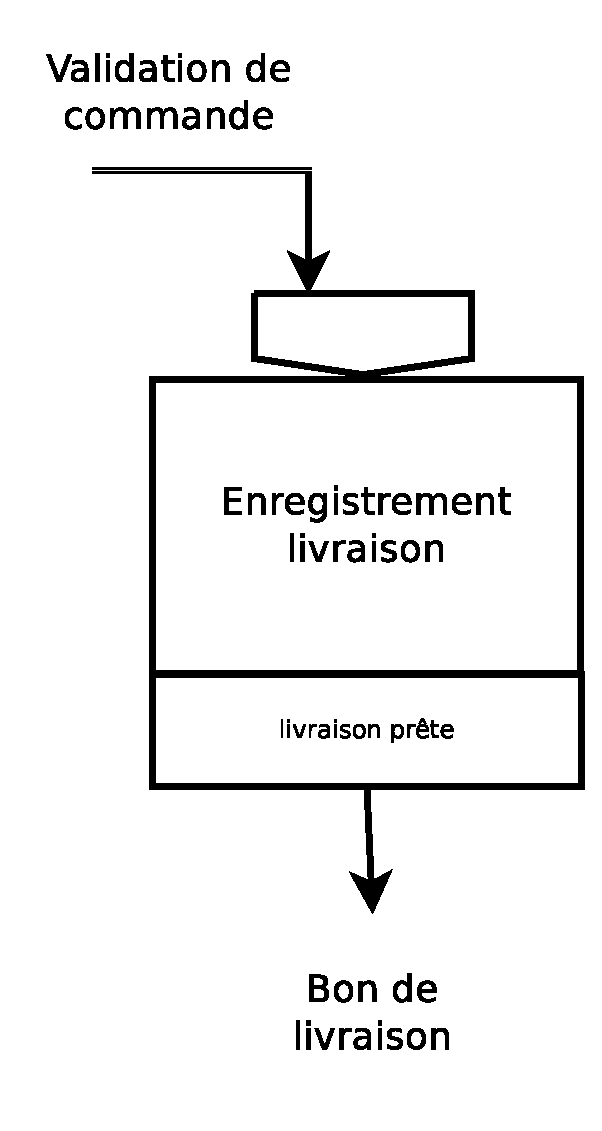
\includegraphics[height=7cm]{images/cc1_mct2.eps}
    \caption{\label{cc1_mct2} Meunier : enregistrer livraison}
    \end{center}
\end{figure}

\begin{figure}[!htb]
    \begin{center}
    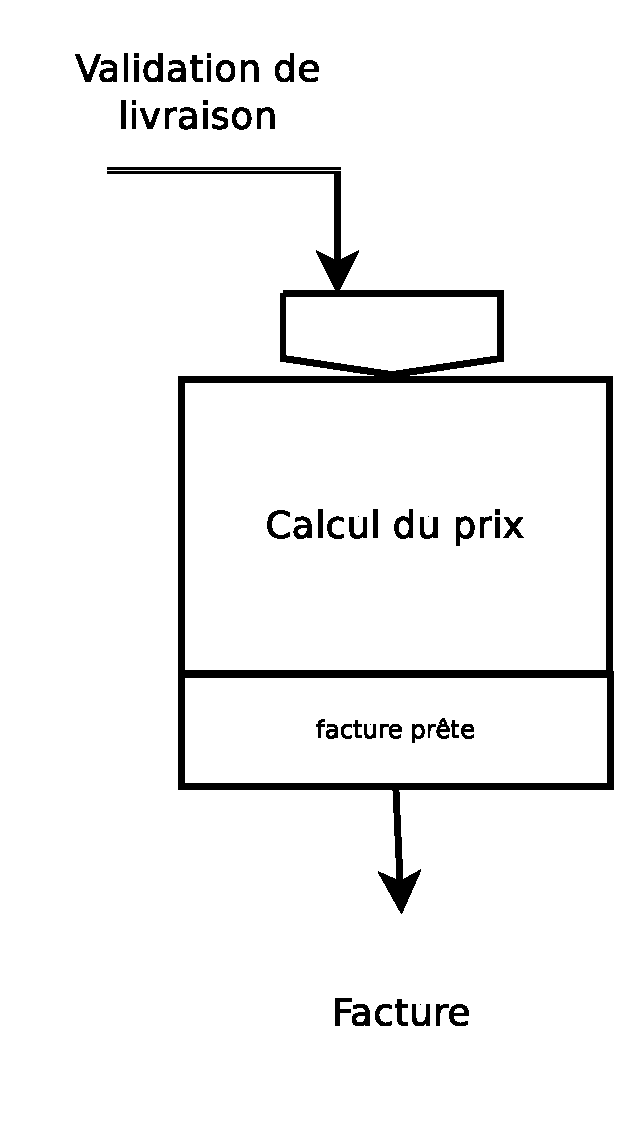
\includegraphics[height=7cm]{images/cc1_mct3.eps}
    \caption{\label{cc1_mct3} Trésorier : Établir facture}
    \end{center}
\end{figure}

\begin{figure}[!htb]
    \begin{center}
    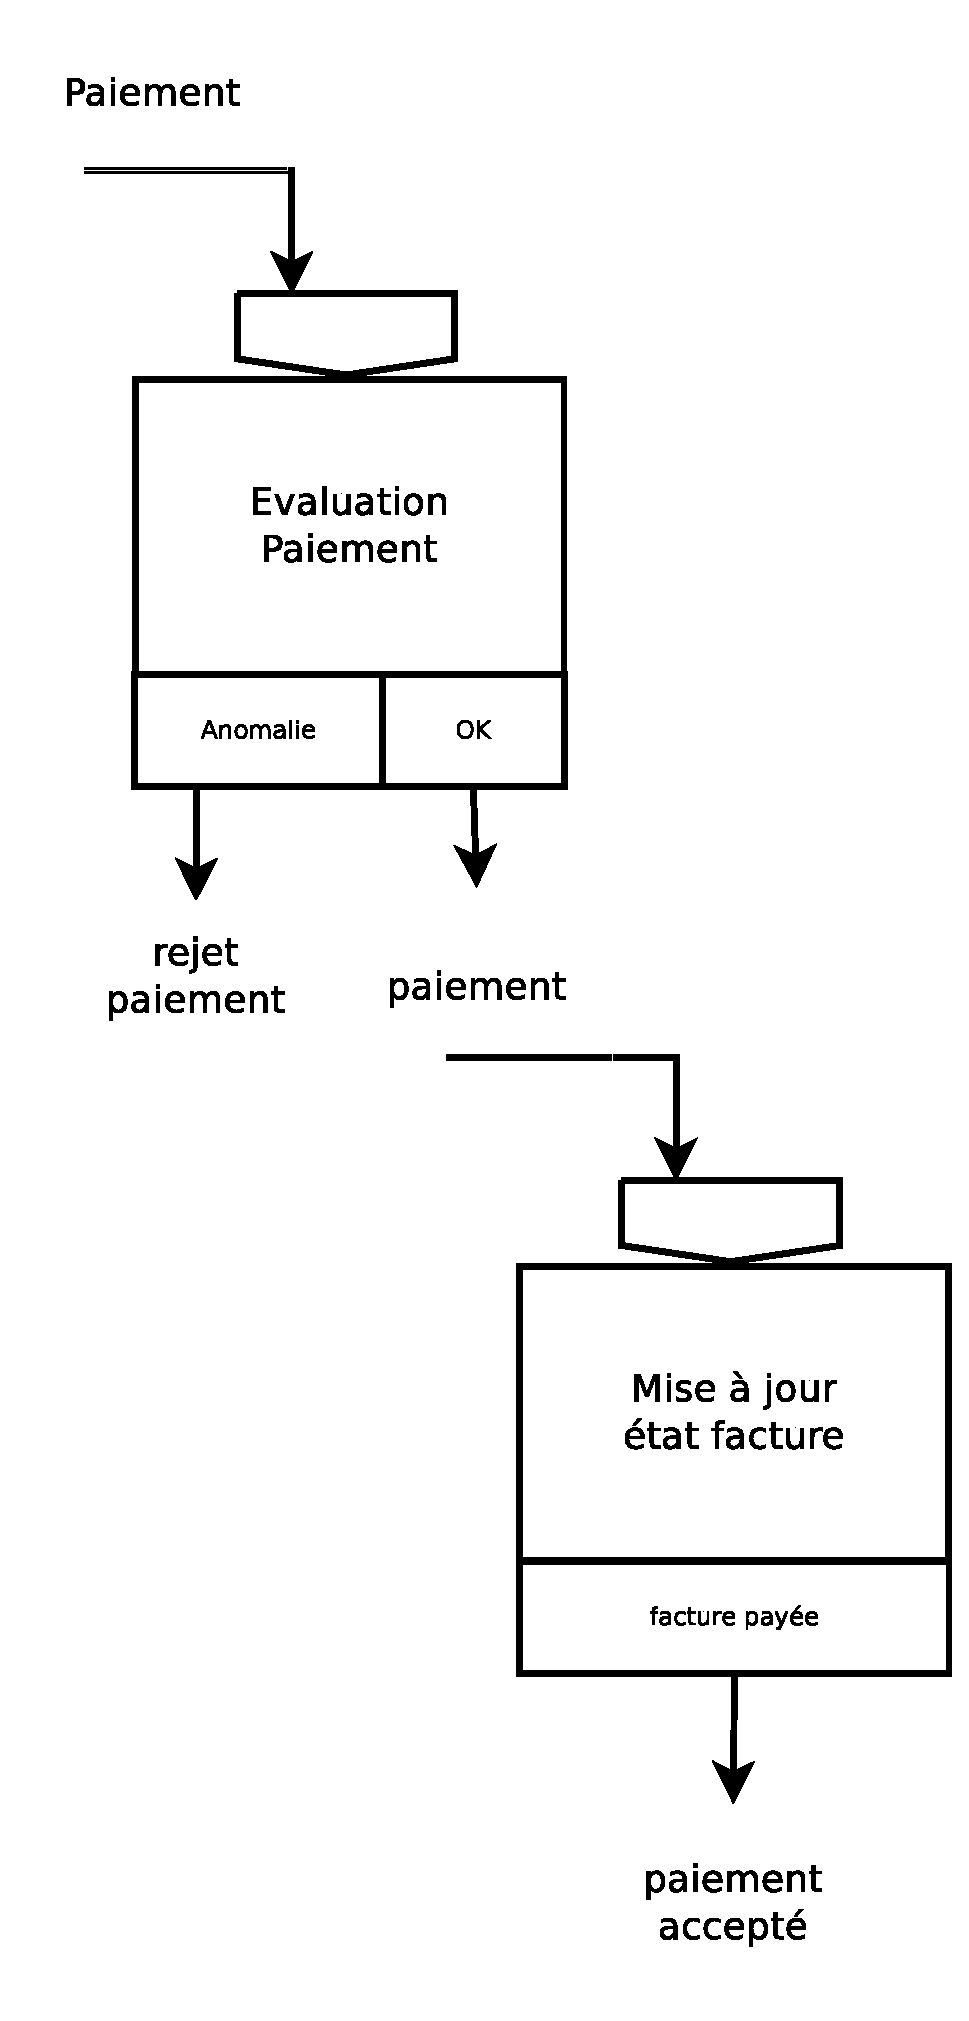
\includegraphics[height=7cm]{images/cc1_mct4.eps}
    \caption{\label{cc1_mct3} Trésorier : Accepter paiement}
    \end{center}
\end{figure}

\newpage
\section*{Modèle Organisationel de Traitements}

On commence par déterminer les différents postes de travail d'utilisation de notre système d'information :\\

\begin{itemize}
    \item
    %\item Bureau du club
    %\item Bureau des homologation
    %\item Bureau de classement
\end{itemize}

\begin{figure}[!htb]
    \begin{center}
    %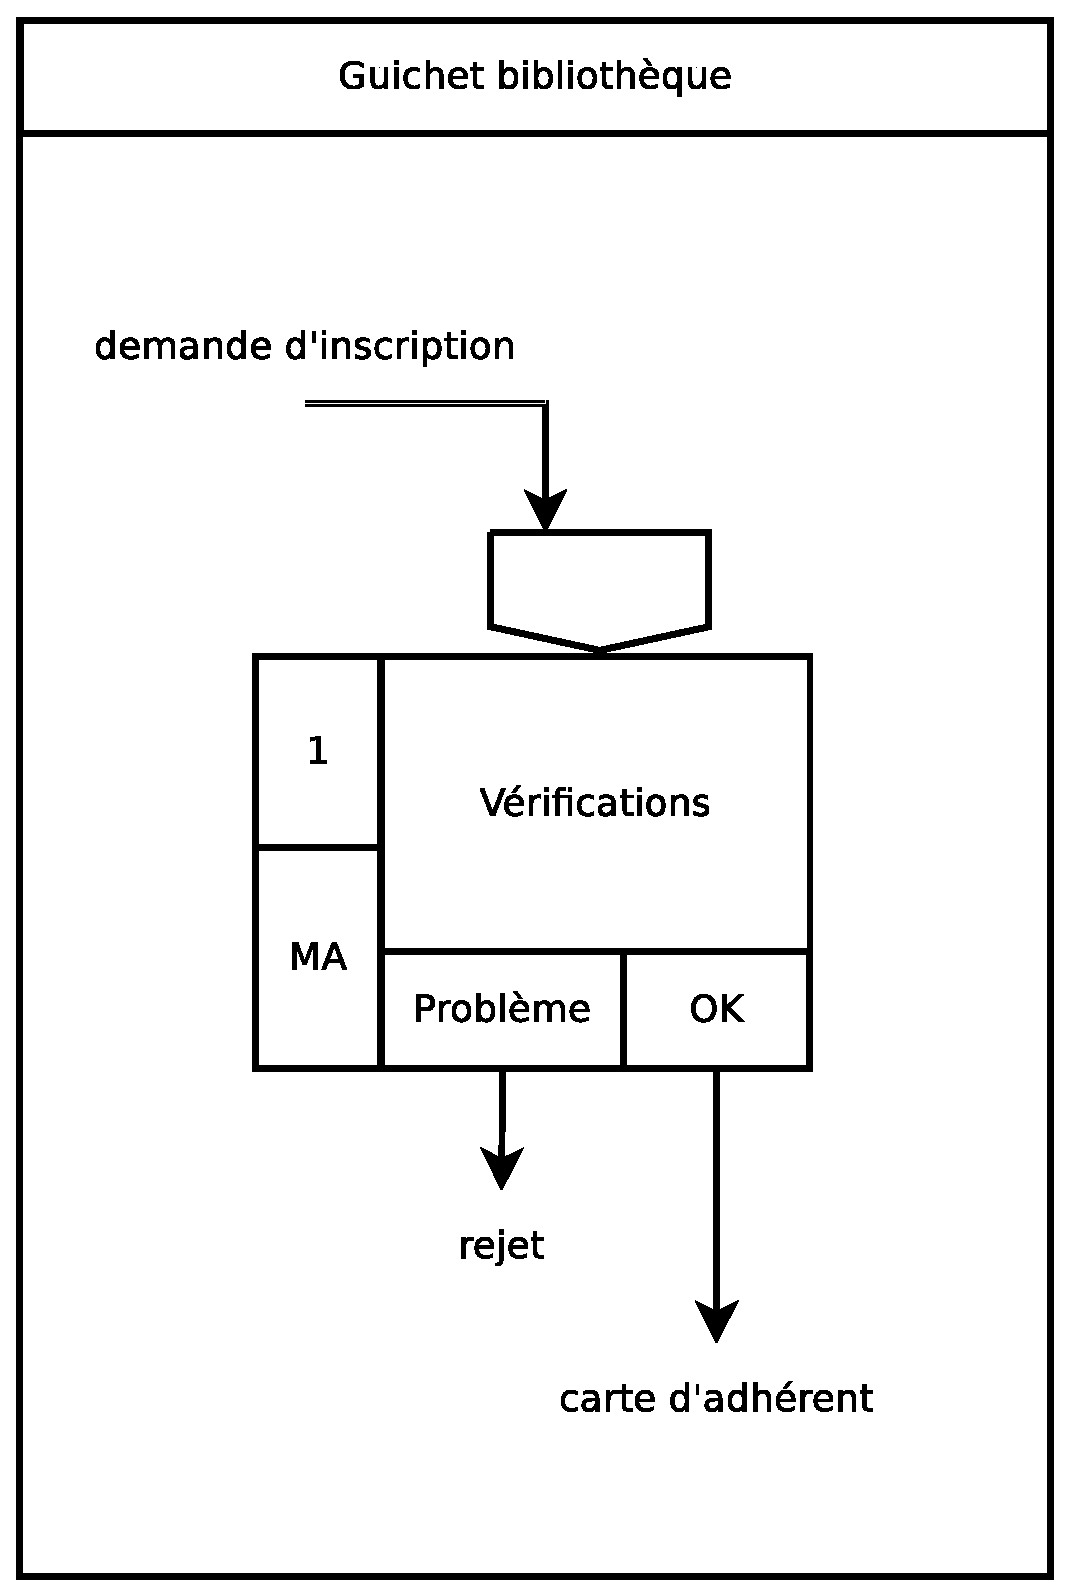
\includegraphics[height=5cm]{images/cc1_mot1.eps}
    %\caption{\label{cc1_mot1} Bureau d'homologation}
    \end{center}
\end{figure}

\begin{figure}[!htb]
    \begin{center}
    %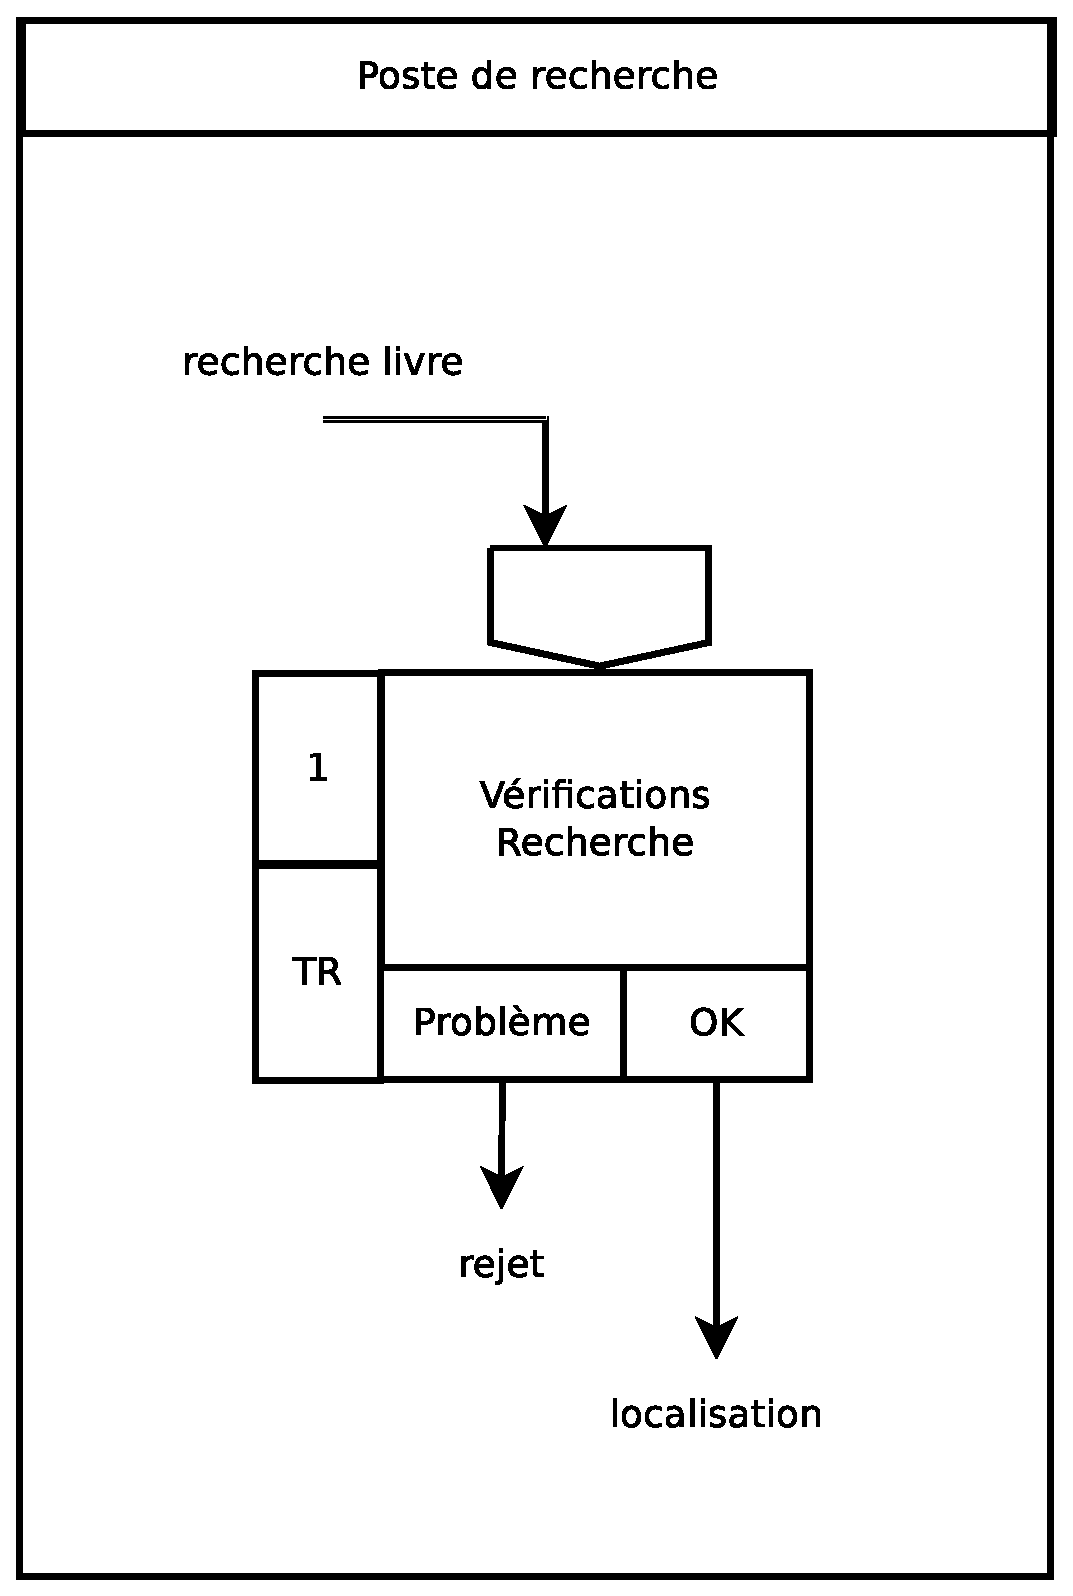
\includegraphics[height=8cm]{images/cc1_mot2.eps}
    %\caption{\label{cc1_mot2} Bureau du club et bureau de classement}
    \end{center}
\end{figure}


\newpage
\section*{Modèle Organisationel de Données}

On commence par déterminer les différents sites de notre système d'information :\\

\begin{figure}[!h]
\begin{tabular}{l l}
%
%
\end{tabular}
    \caption{\label{sites} Sites}
\end{figure}

\newpage
On détermine ensuite les droits d'accès pour les entités et les asssociations porteuses de données :\\

\begin{figure}[!htb]
\begin{tabular}{| l | c | c | c | c | c | c | c | c | c | c | c | c | c | c | c | c |}
%
   \hline
                  & \multicolumn{4}{| c |}{Sec. du club} & \multicolumn{4}{| c |}{Org. de compét.} & \multicolumn{4}{| c |}{Gest. des homolog.} & \multicolumn{4}{| c |}{Gest. du class.} \\
   \hline
                  & C & L & E & S & C & L & E & S & C & L & E & S & C & L & E & S \\
%
\end{tabular}
    \caption{\label{droits} Droits}
\end{figure}

\newpage
On en déduit les modèles d'organisations de données suivants : \\

\begin{figure}[!htb]
    \begin{center}
    %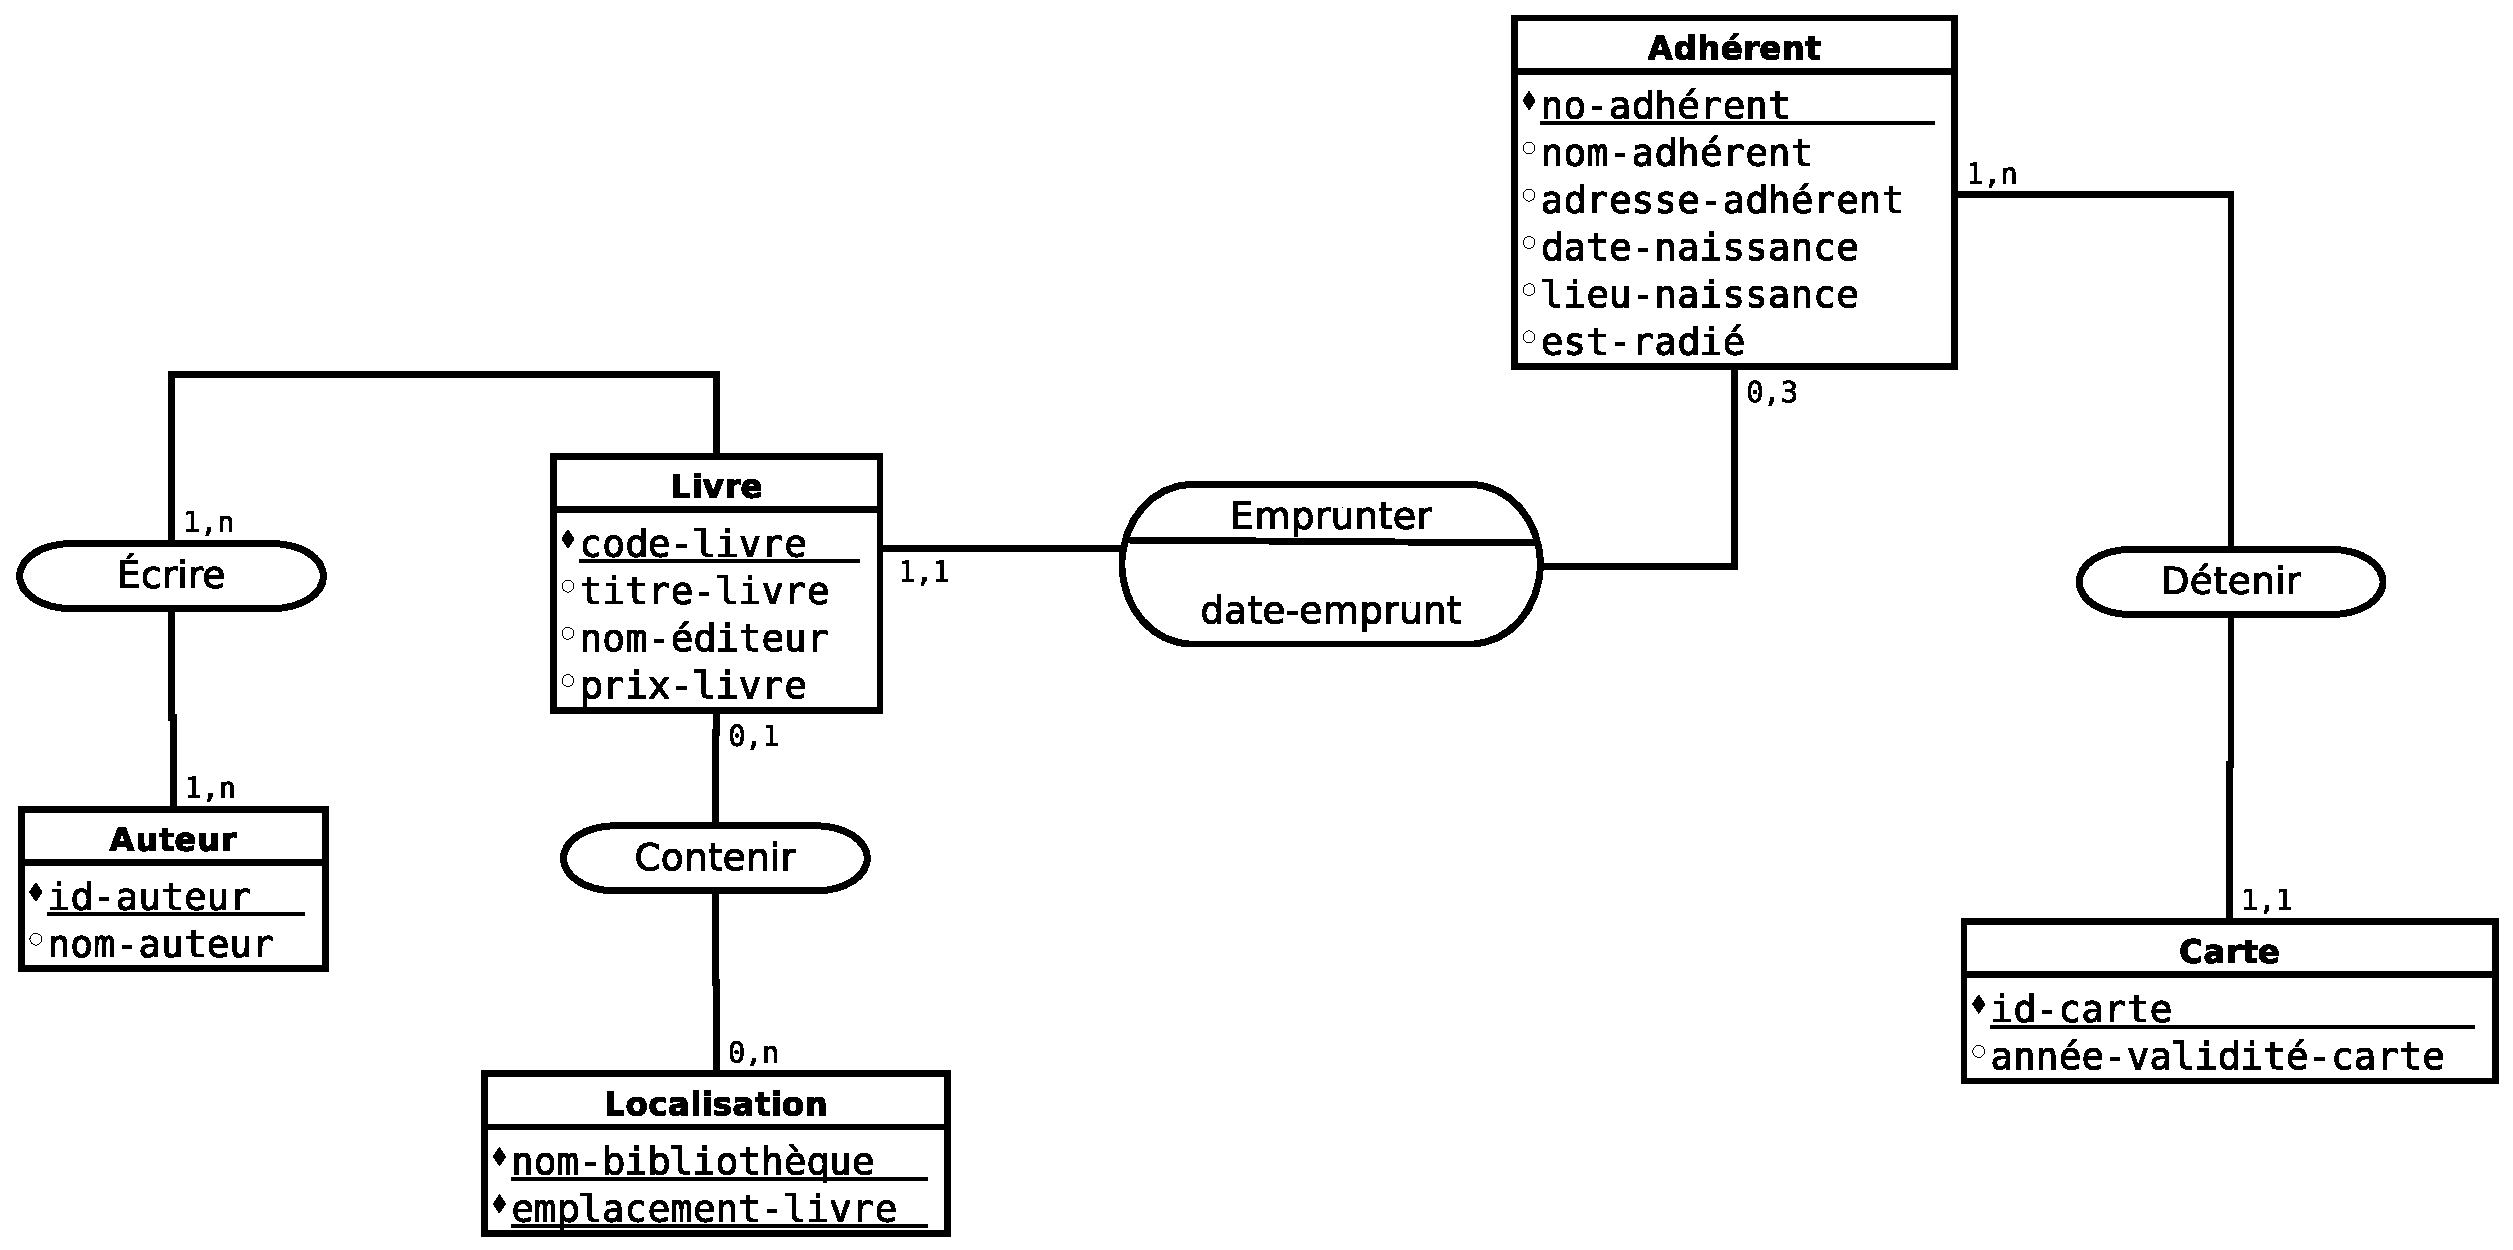
\includegraphics[width=11.5cm]{images/cc1_mod1.eps}
    \caption{\label{cc1_mod1} MOD Salle du club}
    \end{center}
\end{figure}

\begin{figure}[!htb]
    \begin{center}
    %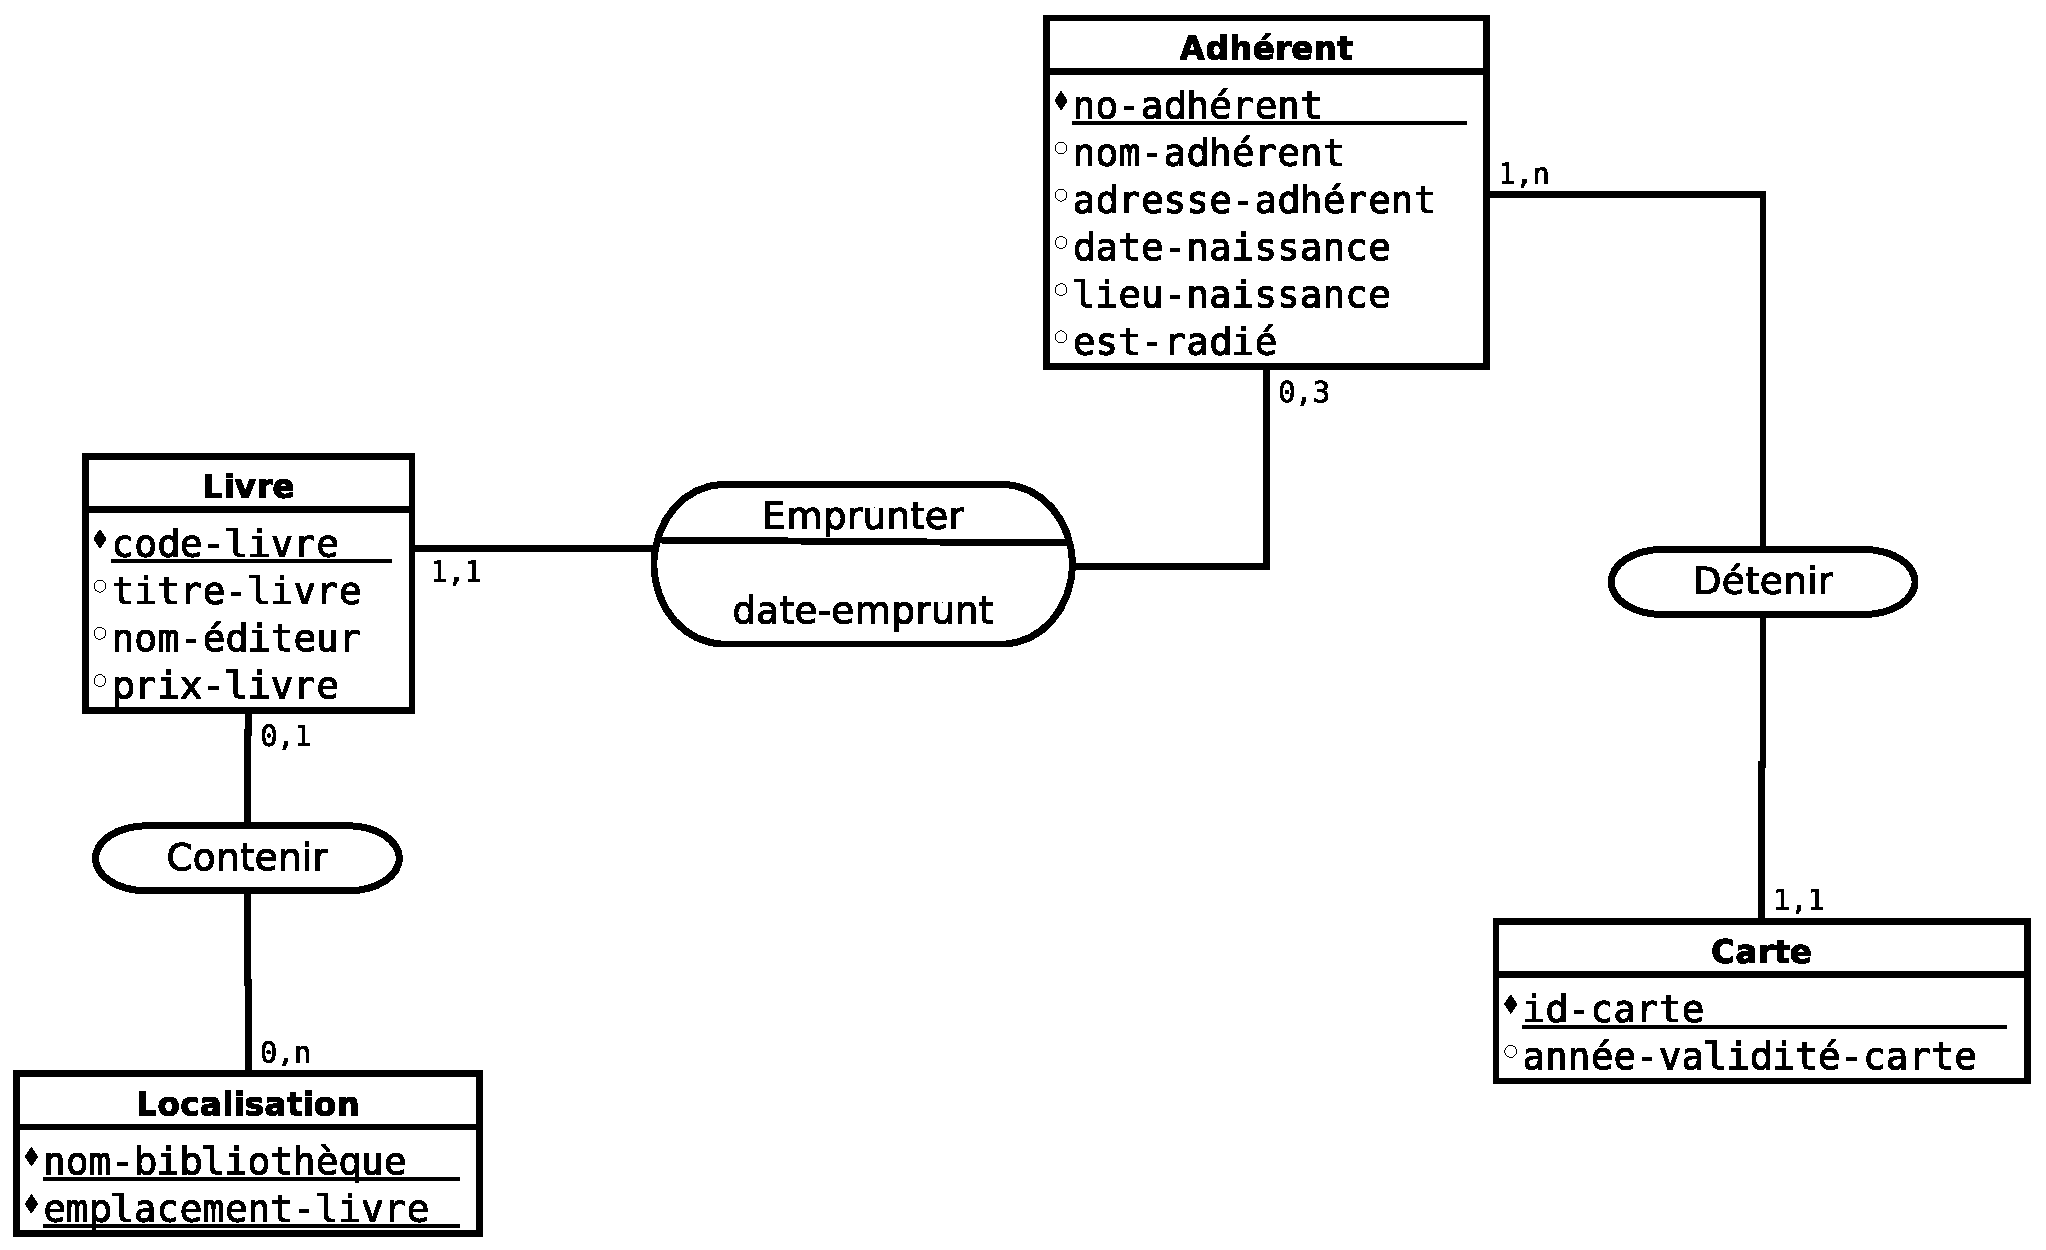
\includegraphics[width=11.5cm]{images/cc1_mod2.eps}
    \caption{\label{cc1_mod2} MOD Siège de la fédération}
    \end{center}
\end{figure}

